\begin{frame}{Exemple: la série Été d'Arte sur Instagram}
    \begin{columns}
    % Colonne de gauche : Texte
        \begin{column}{0.4\textwidth}
            \begin{itemize}
                \item Exemple présenté par \href{https://art-et-reseaux.fr/ete-social-graphic-novel-sur-instagram/}{Nolwenn Tréhondart}
                \item  BD publiée sur Instagram avec la boîte \textit{Bigger than fiction}
                \item Idée est d'introduire de l'art, de la fiction, de la culture et du politique.\\
                \textrightarrow{} Comment capter les utilisateur.rices en respectant les contraintes de la plateforme? 
            \end{itemize}
        \end{column}

        % Colonne de droite : Image
        \begin{column}{0.5\textwidth}
            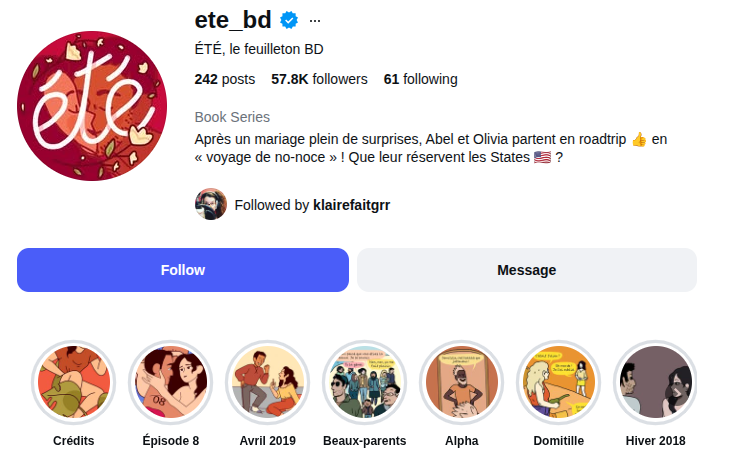
\includegraphics[width=.9\columnwidth]{Images/profil_ete_arte.png}
            
        \end{column}
    \end{columns}
\end{frame}

\begin{frame}{Exemple: la série Été d'Arte sur Instagram}
    \begin{center}
         {\small \textit{ "Les technologies qui permettent d’écouler les marchandises se sont déplacées en une quinzaine d’années du produit au logo, puis du logo aux stories."}}\\
    \textbf{Christian Salmon, \textit{Storytelling, la machine à fabriquer des histoires et à formater les esprits}}
    \end{center}
   
    On cherche des histoires auxquelles on peut s'identifier (\textit{"relatable"}).

\end{frame}

\begin{frame}{Exemple: la série Été d'Arte sur Instagram}
    \begin{itemize}
        \item Chaque épisode doivent se comprendre indépendament des autres.
        \item Respecter la limite de 10 cases par post (au moment de la publication)
        \item Les hashtags sont utilisés comme légende
        \item Mélange de musique, animation et images.
    \end{itemize}
\end{frame}


\begin{frame}{Exemple: la série Été d'Arte sur Instagram}
    \begin{center}
        Cas intéressant: s'adapter à un changement d'algorithme.
    \end{center}
\vspace{1em}
\begin{columns}
    % Colonne de gauche : Texte
        \begin{column}{0.5\textwidth}
            \centering
            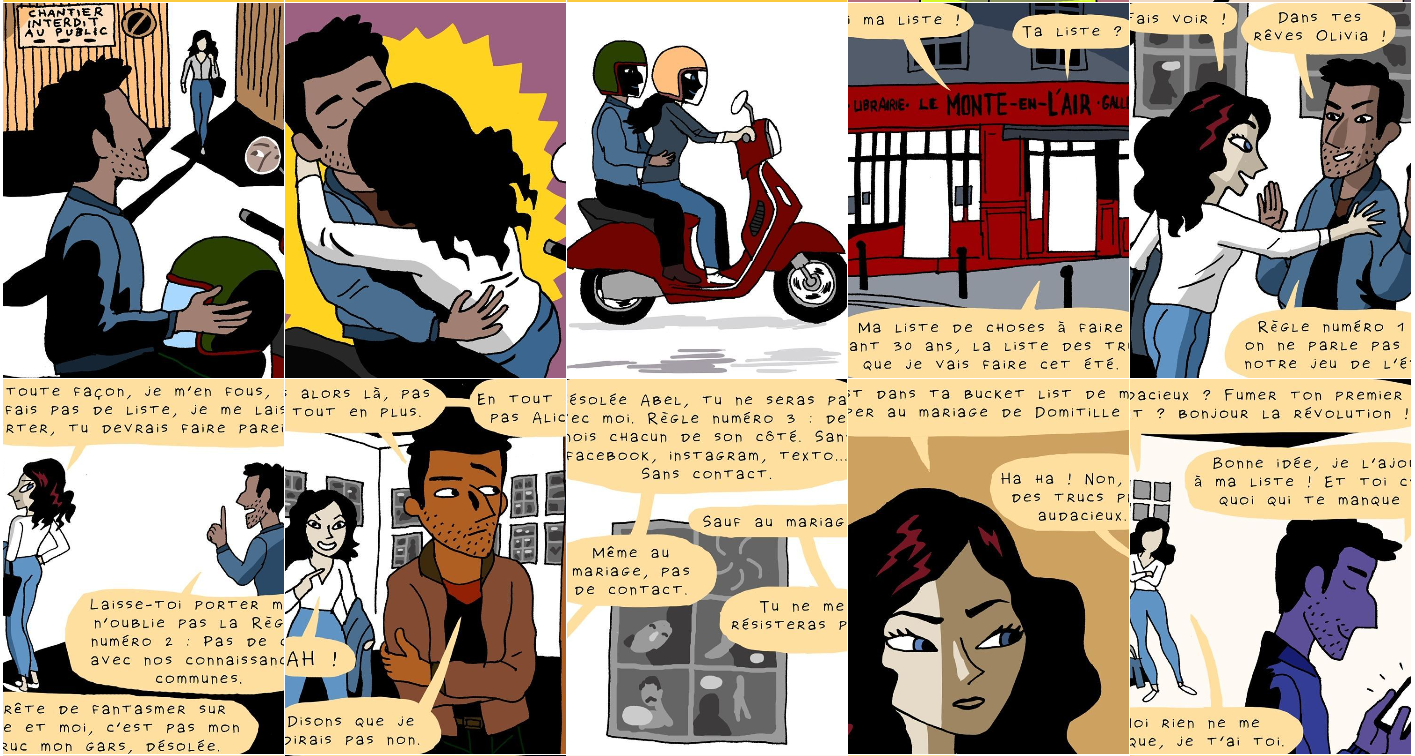
\includegraphics[width=.9\columnwidth]{Images/ete_arte_ancien.png}
            
        \end{column}

        % Colonne de droite : Image
        \begin{column}{0.5\textwidth}
            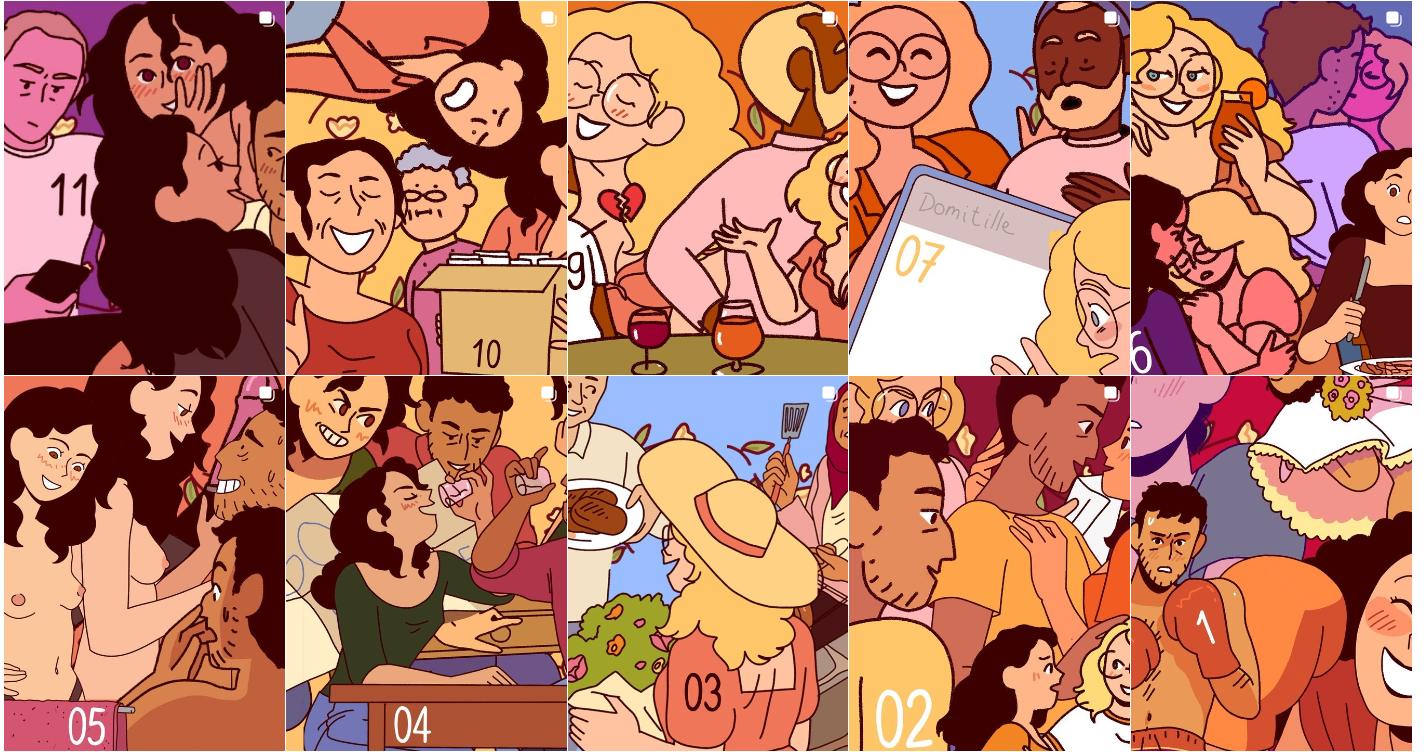
\includegraphics[width=.9\columnwidth]{Images/ete_arte_recent.png}
            
        \end{column}
    \end{columns}

\end{frame}

